\section*{Definition of a Saddle Point}

Consider the autonomous dynamical system $\dot{x} = P(x, y), \, \dot{y} = Q(x, y)$ with an isolated critical point at $(0, 0)$.

\vspace{0.5em}
\noindent The critical point $(0, 0)$ is called a \textbf{saddle point} if:

\begin{enumerate}
    \item There exist exactly \textbf{two trajectories} (separatrices) that approach and enter $(0, 0)$ as $t \to +\infty$ from opposite directions, and \textbf{two trajectories} that enter $(0, 0)$ as $t \to -\infty$ (move away as $t \to +\infty$) from opposite directions.
    \item All other trajectories in the neighborhood of $(0, 0)$ pass near the critical point without entering it and subsequently move away as $t \to \pm\infty$ (forming hyperbolic-like curves).
\end{enumerate}

\subsection*{Eigenvalue Condition (Linear Analysis)}

For the linearized system $\dot{\mathbf{x}} = A\mathbf{x}$, $(0, 0)$ is a \textbf{saddle point} if and only if the eigenvalues $\lambda_1, \lambda_2$ of the Jacobian matrix evaluated at $(0, 0)$ are \textbf{real, non-zero, and have opposite signs}:

\[
\lambda_1 < 0 < \lambda_2 \quad \text{(or } \det(A) < 0\text{)}
\]
\begin{center}
    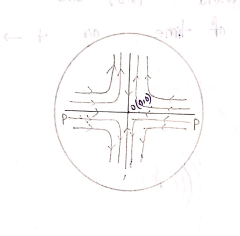
\includegraphics[width=0.5\textwidth]{Image/saddle point.png}
\end{center}
\section*{Definition of a Spiral (or Focus)}

Consider the autonomous dynamical system $\dot{x} = P(x, y), \, \dot{y} = Q(x, y)$ with an isolated critical point at $(0, 0)$.

\vspace{0.5em}
\noindent The critical point $(0, 0)$ is called a \textbf{spiral} (or \textbf{focus}) if:

\begin{enumerate}
    \item Trajectories starting at any point $P$ in a neighborhood of $(0, 0)$ approach the origin as $t \to +\infty$ (stable spiral) or move away from the origin as $t \to +\infty$ (unstable spiral).
    \item Trajectories wind around $(0, 0)$ \textbf{infinitely many times} in a spiral-like manner as they approach or move away from the critical point.
    \item Trajectories \textbf{do not enter or leave along a single well-defined tangent line}, as the direction angle $\theta(t) \to \pm\infty$.
\end{enumerate}

\subsection*{Eigenvalue Condition (Linear Analysis)}

For the linearized system $\dot{\mathbf{x}} = A\mathbf{x}$, $(0, 0)$ is a \textbf{spiral point} if and only if the eigenvalues $\lambda_1, \lambda_2$ of the Jacobian matrix $A$ evaluated at $(0, 0)$ are \textbf{complex conjugates with a non-zero real part}:

\[
\lambda_{1,2} = \alpha \pm i\beta, \quad \text{where } \alpha \neq 0 \text{ and } \beta \neq 0
\]

\begin{itemize}
    \item \textbf{Stable Spiral (Sink):} $\alpha = \text{Re}(\lambda) < 0$ \textit{(trajectories spiral inward toward $(0, 0)$)}.
    \item \textbf{Unstable Spiral (Source):} $\alpha = \text{Re}(\lambda) > 0$ \textit{(trajectories spiral outward away from $(0, 0)$)}.
\end{itemize}
\begin{center}
    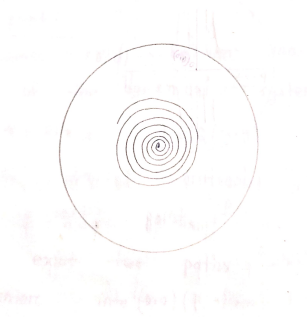
\includegraphics[width=0.5 \textwidth]{Image/spiral.png}
\end{center}
\section*{Definition of a Center}

Consider the autonomous dynamical system $\dot{x} = P(x, y), \, \dot{y} = Q(x, y)$ with an isolated critical point at $(0, 0)$.

\vspace{0.5em}
\noindent The critical point $(0, 0)$ is called a \textbf{center} (or \textbf{centre}) if:

\begin{enumerate}
    \item Every neighborhood of $(0, 0)$ contains a family of \textbf{closed concentric trajectories} (ellipses or circles) enclosing $(0, 0)$ as an interior point.
    \item Trajectories around $(0, 0)$ are periodic and closed, meaning they \textbf{neither approach nor move away} from $(0, 0)$ as $t \to \pm\infty$.
\end{enumerate}

\subsection*{Eigenvalue Condition (Linear Analysis)}

For the linearized system $\dot{\mathbf{x}} = A\mathbf{x}$, $(0, 0)$ is a \textbf{center} if and only if the eigenvalues $\lambda_1, \lambda_2$ of the Jacobian matrix $A$ evaluated at $(0, 0)$ are \textbf{purely imaginary}:

\[
\lambda_{1,2} = \pm i\omega \quad (\text{where } \omega \in \mathbb{R}, \, \omega \neq 0)
\]
\begin{center}
    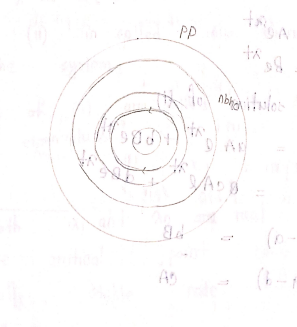
\includegraphics[width=0.4 \textwidth]{Image/center.png}
\end{center}